\begin{figure}[H]
  \centering
  % Primer grafo (G_1)
  \begin{minipage}[t]{0.49\textwidth}
    \centering
    \scalebox{0.7}{% Ajusta este valor (ej. 0.6, 0.7, 0.8) para controlar el tamaño
      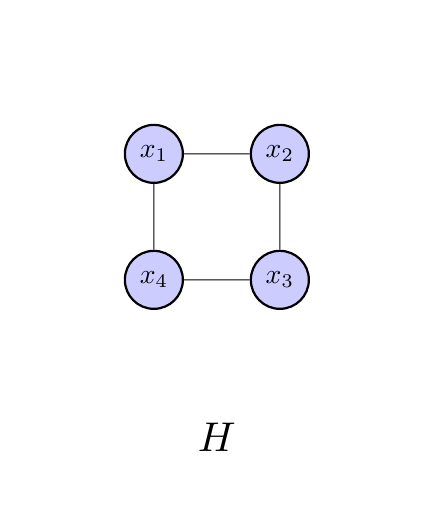
\begin{tikzpicture}[scale=.8,auto=left,every node/.style={circle,fill=blue!20,draw=black,thick}]
  % Vértices del cuadrado interior (C_4)
   \node (w1) at (-1, 1) {$x_1$};
  \node (w2) at (1, 1) {$x_2$};
  \node (w3) at (1, -1) {$x_3$};
  \node (w4) at (-1, -1) {$x_4$};

  % Vértices del cuadrado exterior (C_4 más grande)
  \node (w5) at (-2.5, 2.5) [opacity=0]{$w_5$};
  \node (w6) at (2.5, 2.5) [opacity=0]{$w_6$};
  \node (w7) at (2.5, -2.5) [opacity=0]{$w_7$};
  \node (w8) at (-2.5, -2.5) [opacity=0]{$w_8$};

  % Aristas del cuadrado interior
  \foreach \from/\to in {w1/w2, w2/w3, w3/w4, w4/w1}
    \draw (\from) -- (\to);

  % Título del grafo en la parte inferior
  \node[draw=none, fill=none, scale=1.5] at (0,-3.5) {$H$};
\end{tikzpicture}

    }
  \end{minipage}%
  \hspace{-3.5em}%
  % Segundo grafo (G'_1)
  \begin{minipage}[t]{0.49\textwidth}
    \centering
    \scalebox{0.7}{% Usa el mismo factor de escala para que guarden proporción
      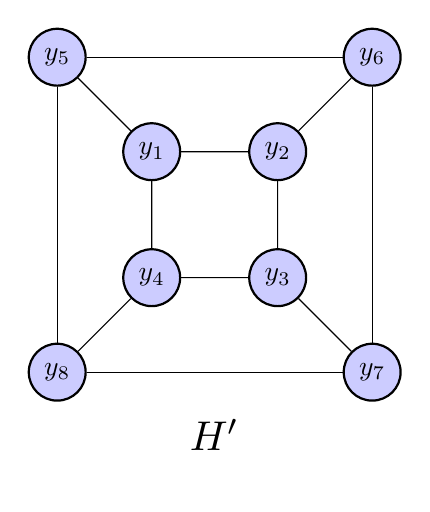
\begin{tikzpicture}[scale=.8,auto=left,every node/.style={circle,fill=blue!20,draw=black,thick}]
  % Vértices del cuadrado interior (C_4)
  \node (w1) at (-1, 1) {$y_1$};
  \node (w2) at (1, 1) {$y_2$};
  \node (w3) at (1, -1) {$y_3$};
  \node (w4) at (-1, -1) {$y_4$};

  % Vértices del cuadrado exterior (C_4 más grande)
  \node (w5) at (-2.5, 2.5) {$y_5$};
  \node (w6) at (2.5, 2.5) {$y_6$};
  \node (w7) at (2.5, -2.5) {$y_7$};
  \node (w8) at (-2.5, -2.5) {$y_8$};

  % Aristas del cuadrado interior
  \foreach \from/\to in {w1/w2, w2/w3, w3/w4, w4/w1}
    \draw (\from) -- (\to);

  % Aristas del cuadrado exterior
  \foreach \from/\to in {w5/w6, w6/w7, w7/w8, w8/w5}
    \draw (\from) -- (\to);

  % Conexiones entre los vértices correspondientes de ambos cuadrados
  \foreach \from/\to in {w1/w5, w2/w6, w3/w7, w4/w8}
    \draw (\from) -- (\to);

  % Título del grafo en la parte inferior
  \node[draw=none, fill=none, scale=1.5] at (0,-3.5) {$H'$};
\end{tikzpicture}

    }
  \end{minipage}
  
  \caption{$\psi$ es un homomorfismo de $H$ en $H'$}
  \label{fig:homomorfismo_grafos_2}
\end{figure}
